%!TEX root = ../thesis.tex
\chapter{Literature Review}
% If you like chapter abstracts ...
\dblspace
\begin{quote}{\em %!TEX root = ../thesis.tex
  In this chapter we discuss previous work examining cardiac anatomy near the cellular scale and its influence on organ-scale function. We first motivate and direct our line of enquiry with experimental evidence, showing how microstructure has a profound effect on propagation dynamics and is central to future antitachycardia pacing treatments. Secondly, we detail the various sources of data available to us to fully characterise this structure, and weigh up their relative advantages and problems. Thirdly, we review the recent attempts to build coherent and geometrically accurate volumes from histology data. Finally, we explore the efforts made in the field to date to incorporate detailed anatomy into models for simulation, again demonstrating the important function of microstructure.

}\end{quote}

\section{Evidence of the Role of Microstructure in Cardiac Electrical Dynamics} % (fold)
\label{sec:microstructure_has_profound_macroscopic_effects_on_propagation_dynamics}
  % Li et al. \cite{Li2010} observed sustained `locally synchronised ventricular fibrillation' in all of 6 dogs, the synchronicity of which they attribute largely to the Purkinje fibres.
  
  \subsection{Vessels, Trabeculae and Papillary Insertions} % (fold)
  \label{sub:vessels_trabeculae_and_papillary_insertions}
    \begin{figure}[htbp]
  		\centering
  		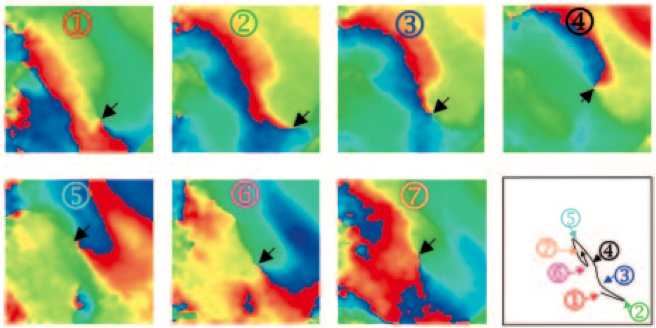
\includegraphics[width=1\textwidth]{Ch4/Figs/valderrabano}
      \caption{A meandering phase singularity from \cite{Valderrabano2003} along a rabbit epicardial artery. Seven sequential phase maps are shown with the trajectory of the singularity in the bottom right. The path is tightly restricted to the underlying artery.}
  		\label{fig:meandering}
  	\end{figure}
    
    It has been known for many years that structure at all scales mediates electrical propagation \cite{DeBakker2006}. Experimental studies demonstrate that microstructure, and specifically vascular and myocardial fibre structure, may be important in arrhythmia mechanisms. Phase singularities are areas of ambiguous activation state surrounded by tissue at all stages of the action potential, present during arrhythmia and fibrillation. They act as the organising centres of reentrant waves \cite{Gray1998}. Optical mapping studies show that phase singularities are restricted around and perpetuated by structural inhomogeneities. In one such study \cite{Valderrabano2003}, singularity clustering was noted in areas surrounding a sharp change or discontinuity in tissue type or fibre direction, such as epicardial vessels, ridges of endocardial trabeculae, and papillary muscle insertions; an example of such behaviour is shown in Figure~\ref{fig:meandering}. In a more recent rat tissue study \cite{Cysyk2008}, controlled placement of a 2-4mm hole (approximately the diameter of the largest vessels in a rat heart) in a homogenous monolayer of cells provides a defined site for wave pinning and excitation during field stimulation. A porcine electrical mapping study \cite{Qin2005} found that only anatomical heterogeneities such as those caused by sub-epicardial vessels were found to stabilise singularities and thus sustain fibrillation for up to 2 hours. Jalife et al. \cite{Jalife2000a} review evidence that ventricular fibrillation may be explained in terms of highly periodic three-dimensional rotors that activate the ventricles at exceedingly high frequency, and that these rotors can remain spatially stable around tissue features.

    During external electrical stimulation of cardiac tissue, secondary sources are induced at tissue inhomogeneities \cite{Sobie1997}, as distinct from the primary electrodes \cite{Roth1998}. In isolated rabbit right ventricular preparations \cite{Ripplinger2006} and in homogenous monolayers of neonatal rat cells \cite{Cysyk2008}, this effect has been exploited to stimulate tissue very near to an anchored phase singularity and unpin the associated spiral wave. In this way, much lower and less traumatic voltages can be applied to the heart to terminate arrhythmia and prevent the onset of fibrillation. These results were reflected in a theoretical study by Takagi et al. \cite{Takagi2004}, which shows that unpinning can be achieved with an electrical stimulus two orders of magnitude weaker than defibrillation energy.
    
    It is worth noting that these studies were limited. The 2D computational study by Takagi \cite{Takagi2004} was simplistic, considering a circular hole in a simplified geometry of isotropic tissue. None of the 2D mapping data obtained offers significant insight into wavefront dynamics below the epicardium or the role played by intramural blood vessels and deeper anatomical anchors in these dynamics. In the longer term, the placement of electrodes and timing of pulses during antiarrhythmic treatment cannot be optimised without accurate knowledge and understanding of reentrant wave propagation that confers real predictive power.
    
  % subsection vessels_trabeculae_and_papillary_insertions (end)

  \subsection{Tissue Type Distribution} % (fold)
  \label{sub:tissue_type_distribution}
    The distribution of ventricular cell and tissue types is also important in the initiation and maintenance of arrhythmia. For example, fibroblasts alter conduction velocity and refractoriness through several mechanisms. Traditionally, only cardiomyocyte decoupling was considered important, where fibroblasts act as passive insulating barriers, creating convoluted ‘zigzag’ conduction pathways and retarding propagation \cite{DeBakker2006,Spach2007}.
  
    Experimental studies have documented that functional gap junctions form between fibroblasts and myocytes \cite{Camelliti2004, Camelliti2005, Walker2007}. Gap junctions affect propagation in three main ways.  Firstly, the conductivity facilitated by the junctions enhances propagation, allowing fibroblasts to transduce activation between otherwise unconnected myocytes \cite{Gaudesius2003, Zlochiver2008}. Secondly and contrastingly, the junctions cause electrotonic loading; fibroblasts act as capacitors coupled to the myocytes, absorbing ionic currents and delaying myocyte activation \cite{Jacquemet2007, Xie2009}. Finally, the coupling elevates myocyte resting membrane potential, causing conduction velocity first to increase and then to decrease with increasing fibroblast concentration and/or gap junction conductance, until finally conduction failure occurs \cite{Miragoli2006, Xie2009}.
  
    Fibroblasts also modulate myocyte behaviour via the release of paracrine factors \cite{Pedrotty2009}. A recent 2D computational study by Xie et al. \cite{Xie2009} suggests that this mechanism adds to the range, complexity and significance of the interaction between the two cell types, whilst conceding that simulating laminar sheet structures using a 2D model may obscure potentially important 3D transfibre effects of the laminar clefts. It went on to say that a real 3D structure is needed for further study, ideally modelled on a realistic representation of 3D cell distribution and coupling.
  % subsection tissue_type_distribution (end)
  
  In short, there are multiple and dynamic interactions between mechano-electrical function and all scales of cardiac morphology, and these are of crucial relevance for normal beat-by-beat activity of the heart, as well as for pathogenesis and therapy. The study of these interactions requires accurate knowledge of cardiac three-dimensional structure, at multiple scales from sub-cellular levels to whole organ. In the next section, we discuss what has been achieved so far toward characterising this structure.
% section microstructure_has_profound_macroscopic_effects_on_propagation_dynamics (end)
  
  \subsection{Myocyte, Fibre and Sheet Orientation} % (fold)
  \label{sub:fibre_direction}
    It is clear that wave propagation is faster parallel to myocytes than perpendicular to them, but there exists great controversy over the three-dimensional arrangement of myocytes within the ventricular walls. Karlon et al. \cite{Karlon1998} automated the quantification of local myofibre disarray in mouse histological sections. Streeter et al. \cite{StreeterJr1969} observed that the myocardial fibres that constitute ventricular tissue are organised such that their angle from the horizontal plane varies transmurally. Much of the literature asserts that the ventricular myocytes are compartmentalized in the form of sheets, albeit that the extent of division, and interrelations, of the sheets is less well explained. Gilbert et al. \cite{Gilbert2007} unify seemingly conflicting features of many of the contemporary structural models, encompassing inter-subject structural variability and proposing the variability as the root source of debate on myocardial architecture. Others present the only muscular unit to be found within the myocardial walls as the cardiac myocyte itself, embedded within an aggregated matrix of fibrous tissue \cite{Anderson2009}. It is also unclear how microstructure reorganises under tissue's own mechanical deformation; ex-vivo DTMRI of hearts at various stages of systole has started to provide insight here \cite{Hales2012}.
  % subsection fibre_direction (end)
  
\section{Cardiac Tissue Can Accurately Be Characterised with High Resolution Images} % (fold)
\label{sec:cardiac_tissue_can_be_accurately_characterised_with_high_resolution_data}
  In this section, we first delineate the various modalities used to image the whole heart: MRI, DTMRI, Q-ball imaging, micro computed tomography, two-photon tissue cytometry and histology. We give an overview of the modelling work carried out with such data so far, and go on to discuss the problems with each modality. We outline how two modalities, either MRI and histology or more recently block face images and histology, can be combined to overcome the failings of each, and what progress has already been made in this regard.
  
  \subsection{MRI} % (fold)
  \label{sub:mri}
    Magnetic Resonance Imaging, or MRI, uses a powerful magnetic field to align the magnetisation of hydrogen nuclei in the imaged medium. Radio frequency fields are then applied in order to perturb the magnetic field, causing the aligned nuclei to process around the energy minimum of the static magnetic field. This procession creates a magnetic field of its own, which is detected by the scanner. Resolutions of up to 26.4 x 26.4 x 24.4$\mu$m have been resolved of rabbit hearts by Burton et al. \cite{Burton2006}, up to 21.5$\mu$m isotropic of rat hearts by Schneider et al. \cite{Schneider2004} and more recently, 25.4 x 25.4 x 12.5$\mu$m in fixed in vitro rat hearts. Recent developments have also shown the possibility of quantifying structure in the myocardium with para-cellular resolution, using contrast-enhanced MRI \cite{Gilbert2012}, in particular in the ex vivo setting. However, in contrast to histological approaches, this does not allow, at present, positive identification of cell size and type.
    
  % subsection mri (end)
  \subsection{DTMRI} % (fold)
  \label{sub:dtmri}
    Diffusion Tensor MRI (DTMRI or DTI) provides a measure for the rate of water diffusion in three perpendicular directions. Six or more diffusion weighted measurements are obtained from different orientations, at each voxel of a single DTI image. A symmetric tensor is then calculated from the data, with three perpendicular eigenvectors whose magnitudes represent the three principal diffusion rates in their respective directions. It has been shown that the three principal axes of diffusion in cardiac tissue are closely aligned with the direction along fibres, perpendicular to fibres within myocardial sheets, and perpendicular to both fibres and sheets \cite{Scollan1998}. The highest resolution obtained with this technique is 101.6$\mu$m isotropic resolution \cite{Bishop2009}.
  % subsection dtmri (end)
  
  \subsection{Q-Ball Imaging} % (fold)
  \label{sub:q_ball_imaging}
    Q-Ball imaging is an established high-angular resolution diffusion MRI technique, which uses MRI measurements taken at a large number of orientations to reconstruct the radially integrated displacement function in all directions at each voxel in the image: the Orientation Distribution Function (ODF). The ODF of a diffusion tensor can be understood as a unit sphere that has been scaled along each of the tensor's three eigenvectors by their associated eigenvalues, to form a spheroid. ODFs from Q-ball imaging, however, can take any form parameterised by orientation (for example, the two angles in spherical polar coordinates), constrained only by symmetry through the origin
    \begin{equation}
      F(\theta, \phi) = F(-\theta, \pi - \phi).
    \end{equation}
    This extra information can be used to discriminate between areas with a single, slowly varying fibre population, rapid fibre rotation and the co-existence of multiple populations of fibres with distinct orientations \cite{Dierckx2009}.
  
  % subsection q_ball_imaging (end)
  
  \subsection{Micro Computed Tomography} % (fold)
  \label{sub:micro_computed_tomography}
    Micro-computed tomography ($\mu$CT) is an emerging, non-invasive imaging modality that allows for non-destructive, high-resolution imaging of tissue \cite{Ragan2007,Deng2012}. It has been shown that $\mu$CT is well-suited for imaging of bones and calcified structures, but it provides low soft tissue contrast. Tissue such as heart muscle therefore requires pretreatment with specific stains or contrast agents. While $\mu$CT provides superior spatial resolution, compared to MRI (typically $<$ 10 $\mu$m \cite{Metscher2009,Stephenson2012}), it cannot resolve cellular composition of tissue.
  % subsection micro_computed_tomography (end)
  
  \subsection{Histology} % (fold)
  \label{sub:histology}
  In the process of histology, an ex-vivo heart can be perfused with various preparatory agents before being gradually infiltrated with wax, over the course of approximately 2 weeks. Once set, the hearts can be serially sectioned, and the resulting slices photographed under microscope. The slices may also be stained with various binding agents in order to visually identify the constituent tissue types. Burton et al. \cite{Burton2006} followed this procedure, obtaining a stack of histology images of resolution 1.1x1.1$\mu$m, with each slice of thickness 10$\mu$m. This  methodology provides the highest resolution and the clearest tissue type distinction of any imaging technique. One major drawback is clear: the positions of the slices within the final images are unrelated.
  
  Despite the rich data that these imaging modalities provide, each technology has its limitations. MRI does not impart any information about fibre direction, and little about tissue type. DTMRI only performs well in areas of uniform, slowly varying fibre direction. Furthermore, DTMRI data is often noisy along surface boundaries due to partial volume effects \cite{Alexander2001}. Dierckx et al. \cite{Dierckx2009} compared Q-Ball imaging with DTMRI, finding good agreement in areas of coherent myofibre direction where diffusion is approximately Gaussian, but large discrepancies where fibres crossed each other, or where there was a sharp change in fibre orientation. In these areas, the Gaussian assumption upon which DTMRI is founded breaks down, and the more general Q-ball approach, mapping an orientation distribution function, is more appropriate. Even so, the spatial resolution of any MRI technique does not currently approach the dimensions necessary to resolve a cardiac cell, of approximately 20 x 20 x 120$\mu$m for myocytes. Individual myocytes can be discerned from histological data, but the method is not only extremely time consuming, but inherently destructive and inapplicable for in vivo measurement. The preparation and fixing methods introduce several deformations from tissue shrinkage during processing, from mechanical forces during the slicing process, and from potentially inhomogeneous relaxation of sections before mounting onto microscope slides \cite{Burton2006}. Moreover, the challenge remains to coregister accurately the 2D slice images once they have been obtained.
  % subsection histology (end)
% section cardiac_tissue_can_be_accurately_characterised_with_high_resolution_data (end)

\section{Cellular-Resolution Tissue Volumes Can Be Reconstructed from Serial Histology} % (fold)
\label{sec:cellular_resolution_tissue_volumes_can_be_reconstructed_from_serial_histology}
  All 3D histology reconstruction methods are based on the acquisition of individual 2D histology images, whether from scans of the un-cut surface of the embedded tissue (so-called block face imaging) \cite{Sands2005,Sands2006,Rutherford2012}, or as sections \cite{Burton2006,Plank2009}. In the former case, 2D images are intrinsically registered, and so no alignment is necessary. In the latter case, images are brought into alignment either through registration amongst themselves, or to a coherent reference volume. It will be seen that the most recent methods draw together the advantages of both techniques.
  
  In 2002, Hooks et al. \cite{Hooks2002} sectioned a 0.8 x 0.8 x 3.7mm transmural segment of rat left ventricle and recorded an intrinsically registered volume image of cubic-1.56$\mu$m resolution using confocal microscopy. The resulting volume images were more detailed than any that had been seen before. Using similar techniques in 2012, Rutherford et al. \cite{Rutherford2012} produced a 5.6mm$^3$ volume surrounding a rat anterior left ventricular infarct, with cubic-1$\mu$m resolution. Unfortunately, this approach cannot resolve tissue sections much larger than the samples presented, and certainly not an entire heart.
  
  It is well documented in the literature that the asymmetrical curvature of an object cannot be recovered solely from a set of two dimensional sections. This issue is known as the `banana problem' \cite{Malandain2004,Lyon2012} or the `z-shift effect' \cite{Yushkevich2006}. Even so, substantial literature is published attempting to reconstruct volumes in the absence of a target geometry \cite{Chakravarty2006,Schmitt2006,Cifor2009,Cifor2011}.
  
  Registering slices to a reference volume circumvents the banana problem. Burton et al. \cite{Burton2006} paved the way for this conjunction by providing MRI rabbit cardiac images of 26.4 x 26.4 x 24.4$\mu$m voxel size with 1.1 x 1.1 x 10$\mu$m histology stacks of the same hearts. They exhibited an initial attempt at slice alignment, guided by the MRI data. First, the difference between adjacent slices was minimised by applying rigid 2D transformations to each slice. Next, they applied a partial differential equation-based approach, solved using a pyramidal and geometric multigrid scheme. While this approach is often used to correct distortion in histological images \cite{Keeling2005}, and is indeed capable of correcting major misalignments, it has an important drawback: by aligning adjacent slices they reduce inter-slice differences that might be fundamental in the description of heart anatomy.
  
  Since then, an automated pipeline has been developed, applying iterative 2D and 3D optimised deformations to register the stacks into the MRI geometry \cite{Mansoori2007}. Histology slices were stacked together into a volume and a rigid 3D transform was optimised to get an initial rough alignment with the MRI volume. Each histology slice was then rigidly registered in its 2D plane with the corresponding MRI slice. Iterations of 3D and 2D registrations are performed until the optimal rigid registration between the two volumes is obtained. In the last stage, non-rigid histology to MRI slice registration was performed using the Demons algorithm \cite{Thirion1995}. Histogram matching was applied as a preliminary step to ensure equal intensities between the two images, as required by the Demons algorithm. Despite some success with this procedure, the slices are ultimately registered to 2D MRI image that does not correspond to the histology, and the unconstrained non-rigid registration that was employed in the final stage led to unrealistic tissue distortions. These problems notwithstanding, the direct registration of histology to MRI is the best way to move towards global shape correctness if no other reference data is available, and is still a common procedure \cite{Alic2011,Osechinskiy2011,Kimm2012}.
  
  Some of the simplest reference-based registration methods rely on manual feature selection or expert hand-drawn atlases. Jagular et al. \cite{Jagalur2007} register thousands of mouse brain histological gene-expression images to expert atlases using automatically selected landmarks. An expert manual approach, whilst appropriate for a quick and approximate result from a small number of data, does not scale, is not repeatable and is prone to human bias.
  
  Block face images, taken from the surface of the fixated tissue volume before sectioning, provide an intrinsically coherent and precisely corresponding set of reference images. Although suitable for low-resolution alignment  \cite{Palm2010}, the reference images are very different in appearance to the histology, with a much lower spatial resolution, hindering accurate alignment. Even very small imperfections in the final mappings introduces jaggedness that renders volumetric microstructure almost imperceptible. Algorithms have been proposed to smooth out this noise through the more precise and reliable coregistration of adjacent slices, in both a sequential \cite{Yushkevich2006,Chakravarty2008} and simultaneous \cite{Feuerstein2011} manner. However, these methods are highly parameterised, often involving registrations at a number of scales, using only a subset of the image information available, and are often based on essentially subjective segmentations, rather than purely original images. Furthermore, only the nearest two neighbouring slices are used to dampen transformational noise, and therefore only the very highest frequency of noise can ever be reduced. Most recently, high-resolution reference images have been provided through the use of two-photon tomography and microtomy \cite{Huang2009,Ragan2012}.
  
  Yushkevich et al. attempt to correct for the banana effect in serially registered mouse \cite{Yushkevich2006} and human \cite{Adler2012} brain histological volumes. They first perform a rigid-body banana registration to approximate the dimensions of a full brain volume. Clearly, if a transform less constrained than rigid-body were used, then each slice would resemble the size and, depending on the constraint of the transform, the shape of the first reference slice. A prism-like volume would result, entirely unrelated to the true geometry of the organ. Yushkevich et al. obtain resampled 2D MRI images corresponding to each section via a rigid 3D registration of the MRI to the z-shifted histology. The volume produced from registering each section to these MRI images is jagged, and so the transformation parameters are Gaussian smoothed to recover some of the continuity of the serial volume. This approach goes a long way to combining the global fidelity of anchoring to a reference volume and the local smoothness of adjacent slice registration. Yet smoothness is limited by the level of success of the individual inter-slice registrations; any error or discontinuity in the serial volume will be transduced directly into the final result. In particular, any differential deformation of adjacent slices during sectioning, either affine or curved, could not be resolved by the rigid-body banana registration, and would manifest as disjoints through the tissue in the z-direction. Moreover, they themselves concede that the method entails a great deal of empirical parameterisation and manual intervention, from the slice segmentation, to the graph edge weighting of the adjacent slice selection, to the width of the Gaussian smoothing of the histology-to-MRI transform parameters.
  
  No mention of non-rigid transforms is mentioned in the Yushkevich implementation. But conceivably, non-rigid interslice registrations could be integrated into the pipeline once the MRI correspondence planes had been established, initialised from the terminus of the rigid registrations. In this case, one would be faced with two disagreeable alternatives. On the one hand, a direct registration could be performed from each slice in the cylindrical, non-rigid banana volume to the reference volume. In this case, most of the slices would be so distant in size, shape and position from alignment with the reference slice as to preclude consistent, successful registration. A better solution would be to apply the Gaussian smoothing to the transforms from the non-rigid, prism-like banana volume to the reference volume. These transforms could be computed by composing the inverse of the transforms from the rigid banana volume to the non-rigid volume with the transforms from the rigid banana volume to the reference volume. Volumes would certainly be smoother than with the rigid smoothing, as adjacent non-rigid differences have been relaxed. Yet unnecessary errors and inaccuracies in alignment would still be present, as slices are only given one algorithmic run to align, and it is implausible that the freedoms inherent in the transform of choice exactly correspond to the distortions undergone by the tissue sections.
  
  Chakravarty et al. \cite{Chakravarty2008} first rigidly align sections of whole mouse brain to an associated block face set, then apply a deformation field transformation to each slice, calculated as the mean of the parameters from defomation fields registering it to the two neighbouring slices. While this may go some way to reducing noise from the block face registrations, the maximum distance of information transfer is one slice, and so only the maximum distortion frequency will be damped.
  
  Techniques have been developed to combine monomodal adjacent slice and multimodal reference registrations simultaneously. Palm et al. \cite{Palm2008} expound a `weighted multi-image mutual information metric', optimising the sum of scaled contributions from both cost functions, and Feuerstein et al. \cite{Feuerstein2011} combine two potential energy functions in a Markov random field model to reconstruct a rat kidney. Not only do these methods require extraneous parameterisation and tuning, but in practice, the superposed cost function will form several distinct local minima; rather than reaching an averaged compromise between the reference images, the optimisation will arrive close to one preferred of several single-image minima, depending on the relative weightings and the transform initialisation.
  
  Atlases of both histology and MRI have been constructed by averaging histological volumes \cite{Li2009}, which were registered based on the approaches taken by \cite{Malandain2004,Yushkevich2006}. Having segmented mouse brain sections, their centres of mass were aligned and a rigid body registration was performed between adjacent slices. The banana effect was mitigated by a 3D registration to MRI, a slice-wise alignment of histological centres of mass to their MRI cross-section equivalent, and a final 3D non-rigid registration. Whilst perhaps appropriate for such low resolution data as presented, these methods are heuristic at best, and introduce several artificial sources of distortion.
  
  Finally, \cite{Arganda-Carreras2010} offer an interesting and robust approach to combining monomodal and multimodal alignments, using consistent b-spline-based elastic registrations. Multiple iterations of triple-wise registrations gradually share information in the z-direction and result in smoothing through a spectrum of scales. However, the choice of simultaneous registration leads to the same problem of multiple local minima faced by \cite{Palm2008,Feuerstein2011}.
% section cellular_resolution_tissue_volumes_can_be_reconstructed_from_serial_histology (end)

\section{The State of the Art in Modelling and Simulation Incorporates Microstructural Detail} % (fold)
\label{sec:the_state_of_the_art_in_microstructural_modelling_and_simulation_incorporates_microstructural_detail}
  Imaging techniques, image processing algorithms, mesh generation software \cite{Prassl2009} and simulation environments have been developed and woven together in recent years to model the electrical, and increasingly electromechanical, behaviour of the heart; the scope for detailed, rigorous and accurate modelling and simulation is widening. In this project, some of the most advanced toolkits available have been used, including ITK. Tarantula (www.meshing.at) is a proprietary program for generating tetrahedral meshes from volumetric data, used in several models of cardiac tissue \cite{Bernabeu2008,Bishop2006,Plank2009}. Two leading simulation environments, The Cardiac Arrhythmia Research Package (CARP, \cite{Vigmond2003}) and Cancer, Heart And Soft Tissue Environment (CHASTE, \cite{Pitt-Francis2008, Pitt-Francis2009, Pitt-Francis2009a}) have enabled large-scale electrophysiological simulations to be run on high performance computing facilities \cite{Bernabeu2008}.
  
  Computational models are increasingly being applied as a way to link spatio-temporal scales, complementing traditional “wet-lab” approaches and projecting between bench and bed-side \cite{Hunter2010,Kohl2010}. An abundance of three-dimensional anatomical models of the cardiac ventricles and atria have been constructed \cite{Eason1998,Kanai1995,Vetter2005,DeBakker2005,Atkinson2011,Baher2011,Bishop2009,Bishop2012,Bordas2010,Bordas2011,Deo2009,Keller2012,Moreno2011,Niederer2011,Okada2011,Potse2006,Romero2010,Seemann2006,TenTusscher2007,Trayanova2011,Vadakkumpadan2010,Zemzemi2011,Zhao2012,Plotkowiak2008}. Accurate microstructural information such as fibre direction is very difficult to obtain, and many of these models include it in a non-specific, rule-based way \cite{StreeterJr1969}. Some models of microstructure have been implemented with information acquired from high-resolution imaging modalities including DTMRI. The reader is referred to previously published reviews of specific areas of computational cardiac electrophysiology \cite{Rudy2006,Brennan2009,Clayton2010,Clayton2011,Greenstein2011,Trayanova2011,Carusi2012}. The simulations based upon all of these models have provided unprecedented insight into the relationship between cardiac structure and function.

  % Fiber architecture is usually incorporated into tissue models by extracting information from histological or diffusion tensor-MRI images using image processing algorithms or using a mathematical rule that relates fiber rotation at a particular location with distance to the surfaces of the ventricular wall (43, 51, 77, 103, 111).
    
  Hooks et al. \cite{Hooks2002} opened a new direction in detailed image-derived 3D cardiac modelling. They manually constructed a finite element mesh from a volume image of a transmural rat heart segment.  Discontinuous bidomain simulations demonstrated for the first time that the laminar organisation of cardiomyocytes into sheets determines unique electrical properties tangential and normal to the sheets. Furthermore, interlaminar clefts between layers of myocytes were seen to act as secondary sources of electrical activation when an external shock is applied. The results were experimentally corroborated in a later study by the same group \cite{Hooks2007}, where arrays of intramural plunge electrodes measured voltage after stimulation in live pigs. The hearts were then removed, treated, frozen and histologically sectioned. The model of the reconstructed histology formed the basis of the subsequent conductivity tensor estimations.
  
  In 2006, Potse et al. \cite{Potse2006} pioneered whole-heart simulations based on MRI data with a rule-based muscle fibre direction, in order to compare monodomain and bidomain ionic models. In bidomain models extended to include fibroblasts \cite{Sachse2009}, increased myocyte-fibroblast coupling and fibroblast-myocyte ratio reduced peak voltage and maximal upstroke velocity of myocytes as well as amplitudes and maximal downstroke velocity of extracellular potentials. The most up-to-date models are now including a wealth of geometrical and structural information derived from high resolution MRI and histology imaging datasets. Xie et al \cite{Xie2004} investigate the interaction between fixed heterogeneities and dynamical instabilities in fibrillation in a canine cardiac geometry with DTMRI-based fibre orientation. Bishop et al. \cite{Bishop2009} highlight the utility of histoanatomically detailed models for investigations of cardiac function, in particular for future patient-specific modelling. They compared simulations from two rabbit heart meshes derived from the same MRI data, with one including finer detail and structure, such as trabeculae and blood vessels. It is observed that trabeculae act as stimulation short cuts, and vessels act as virtual electrodes to damp external stimulation. In another study \cite{Bishop2009a}, they compare fibre directions obtained from DTMRI with those from a rule-based algorithm in rat, and found a close overall match between simulations based on the two models. Overall, the inclusion of anatomical detail, when compared to lower resolution models, alters simulated wave propagation both locally and globally.

  Including details such as blood vessels as well as accurately representing the fibre structure around and within them might be important in understanding the complex morphology of intramural wavefronts beneath the epicardial surface. Some \cite{Ding2001,Hyatt2003} have suggested how surface-recorded optical signals can provide information regarding the sub-surface wavefront propagation direction, although how well this technique relates to more complex anatomical models has been disputed \cite{Bishop2006}. The inclusion of extra anatomical detail, such as vessels and the complex fibre structure around them, may influence wavefront morphology as well as affecting the surface-recorded optical mapping signal.
  
  We have seen that computational modelling techniques can provide a unique window of inference into true 3D propagation. Hitherto however, those models have not included an accurate representation of myocardial fibre orientation, neither do they incorporate high-resolution tissue type mapping. Images of the quality necessary to resolve this detail have been made available, and it is now possible to integrate the information they provide into our modelling and simulation frameworks.
% section sec:the_state_of_the_art_in_microstructural_modelling_and_simulation_incorporates_microstructural_detail (end)

\section{Conclusion} % (fold)
\label{sec:conclusion}
  In summary, microstructure is central to certain mechanisms of arrhythmia, and elucidating the nature of its contribution may eventually aid the diagnosis and treatment of heart disease. Images of the quality required to resolve microstructure are now available. Coherent, full-colour, cellular-resolution, whole-organ, histological tissue volumes can be reconstructed, and microstructural properties can be extracted, using the latest imaging algorithms and techniques. However, these methods all have their own weaknesses. The results of simulations incorporating the newly resolved structure offer a path of insight into the mechanisms of arrhythmia.
% section conclusion (end)
